\chapter[~]{Знайомство з базовими можливостями системи КОМПАС-3D}

\textbf{Мета роботи} --- ознайомитись з основними прийомами роботи в програмному пакеті підготовки
конструкторської документації КОМПАС-3D, навчитись виконувати креслення простих деталей на площині.

\section{Короткі теоритичні відомості}

\textbf{Система КОМПАС-3D} --- інтерактивний графічний редактор з сучасним інтерфейсом, оснащений
інструментальними засобами, які дозволяють створювати твердотілі об'єкти з використанням набору
елементарних параметричних тіл (паралелепіпед, циліндр та ін.)

Просторові твердотілі та каркасні моделі об'єктів (деталей, вузлів, виробів, будівель і т. п.) при
виконанні проектно-конструкторських, технологічних та дизайнерських робіт в машинобудуванні,
приладобудуванні, будівництві, архітектурі).

\subsection{Бібліотеки для КОМПАС}
\subsubsection{Бібліотека анімації}
Бібліотека анімації є стандартним застосунком для КОМПАС-3D. Вона працює з версіями КОМПАС-3D V8 і
вище. Додаткових модулів (окрім самого КОМПАС-3D) для роботи додатку не потрібно. Бібліотека
призначена для імітації руху (анімації) виробів, розроблених у системі тривимірного твердотільного
моделювання КОМПАС-3D. Бібліотека дозволяє:

\begin{itemize}
\item Імітувати рухи складових частин виробу в процесі реальної роботи (можуть використовуватися
  сполучення деталей, що накладаються користувачем у процесі проектування 3D-збірки). Для цих цілей
\item Бібліотека дозволяє задавати як переміщення компонентів, так і їх обертальний рух.
\item Автоматично перевіряти можливі колізії (зіткнення деталей) у процесі руху для виявлення
  помилок у проектуванні.
\item Наочно імітувати процес «розбирання-збірки» виробу для застосування в інтерактивному
  електронному технічному керівництві.
\item Створювати діаграму послідовних положень механізму — «кінограму» (набір послідовних кадрів у
  форматі *.frw — фрагмент КОМПАС-Графік).
\item Записувати відеоролик руху у форматі *.avi. Відтворення можливе як на поточному кроці
  анімації, так і в цілому.
\end{itemize}

Анімація складається з послідовних кроків. На кожному кроці можна задавати різні види
руху деталей і параметри руху (швидкість, частота обертання, час). Сценарій процесу анімації
зберігається в текстовому файлі стандартного XML-формату. Бібліотека анімації не тільки значно
підвищує якість проектування виробів в цілому, його наочність і зручність, але також підсилює
конкурентоспроможність підприємства на етапах виконання конкурсних проектів.

\subsubsection{Бібліотека фотореалістики}
Бібліотека призначена для створення фотореалістичного зображення тривимірної моделі деталі або
збірки, спроектованої в КОМПАС-3D. Бібліотека фотореалістики дає можливості для створення 244
ефектних зображень виробу і використання їх у презентаціях і рекламній документації. Для зручності
роботи в бібліотеці реалізований режим інтерактивного рендерінга, що дозволяє здійснювати попереднє
відображення моделі з текстурами, призначеними в сцені. Матеріали:

\begin{itemize}
\item Вибір матеріалів з широкого списку вбудованої бібліотеки (різні види металів, дерева, каменя,
  пластика та багато інших).
\item Настройка властивостей матеріалу, таких як колір поверхні, що відображає здатність,
  дзеркальність, прозорість, шорсткість і текстура.
\item Можливе призначення матеріалів збіркам, деталям, операціям і поверхням.
\item Реалізований попередній перегляд матеріалів, сцени і джерел світла для зменшення часу
  отримання фотореалістичного зображення.
\end{itemize}

\section{Виконання роботи}

Згідно з варінтом для побудови була задана наступна деталь:

\begin{figure}[!ht]
  \centering 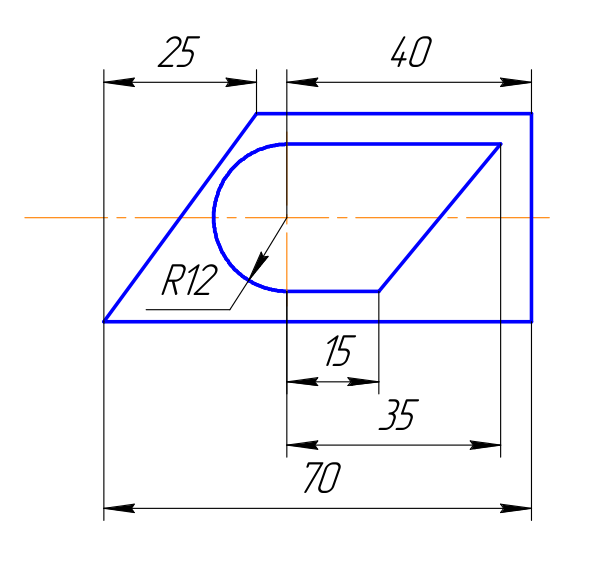
\includegraphics[width=0.9\linewidth]{./images/lab3/target-part.png}
  \caption{Задана деталь для побудови}
  \label{fig:lab3:target_part} 
\end{figure}

\begin{enumerate}[leftmargin=*]
\item За допомогою інструменту ``Прямокутник'' будуємо відповідну фігуру і задаємо необхідні розміри
  (\ref{fig:lab3:rectangle}).
  \begin{figure}[!ht]
    \centering 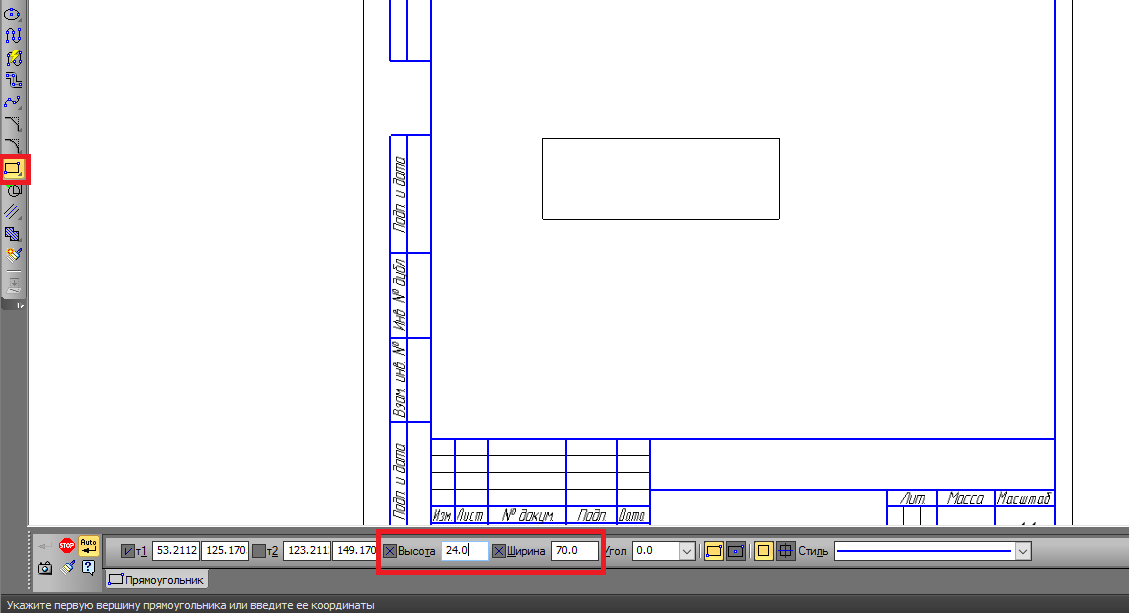
\includegraphics[width=0.9\linewidth]{./images/lab3/step1.png}
    \caption{Застосування інструменту прямокутник}
    \label{fig:lab3:rectangle} 
  \end{figure}

\item За допомогою інструмента ``Автоматичний розмір'' проставляємо розміри деталі
  (\ref{fig:lab3:dimentions}).
  \begin{figure}[!ht]
    \centering 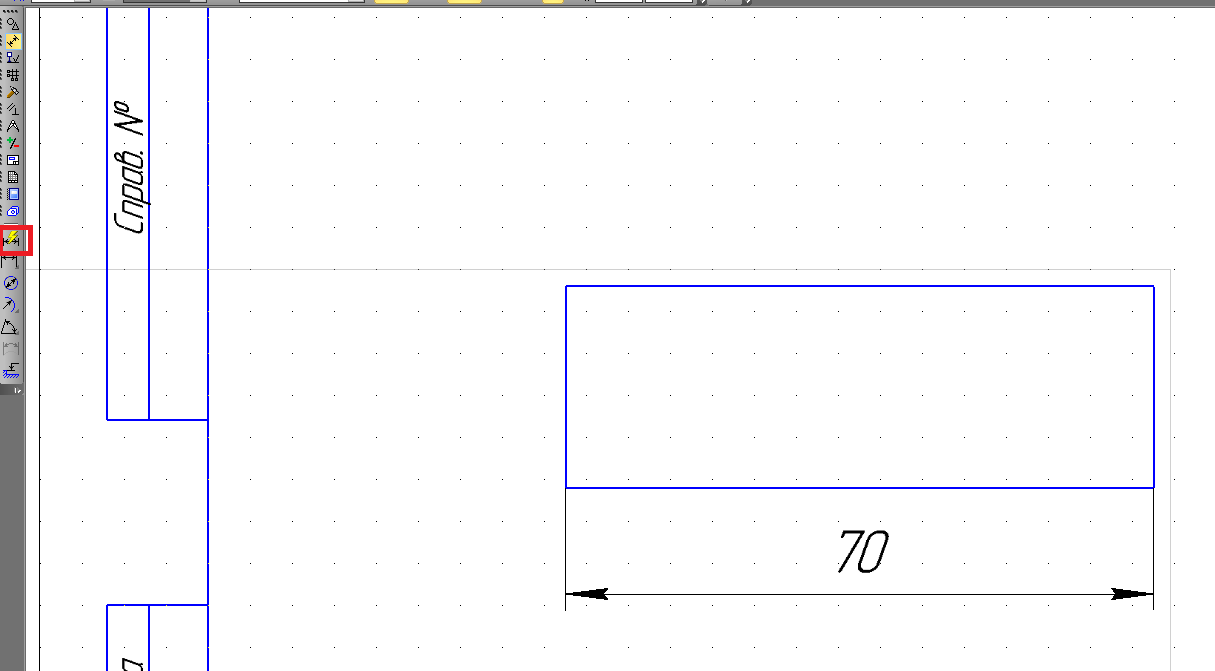
\includegraphics[width=0.9\linewidth]{./images/lab3/step2.png}
    \caption{Застосування інструменту ``Автоматичний розмір''}
    \label{fig:lab3:dimentions} 
  \end{figure}
\item Видліяємо стоврений прямокутник, і вибираємо в контестному меню (викликається правим кліком
  мишки) пункт ``Зруйнувати'' \textit{(``Разрушить'')}, щоб розділити об’єкт на відрізки
  (\ref{fig:lab3:dismantle}). Після чого формуємо необхідний контур.
  \begin{figure}[!ht]
    \centering 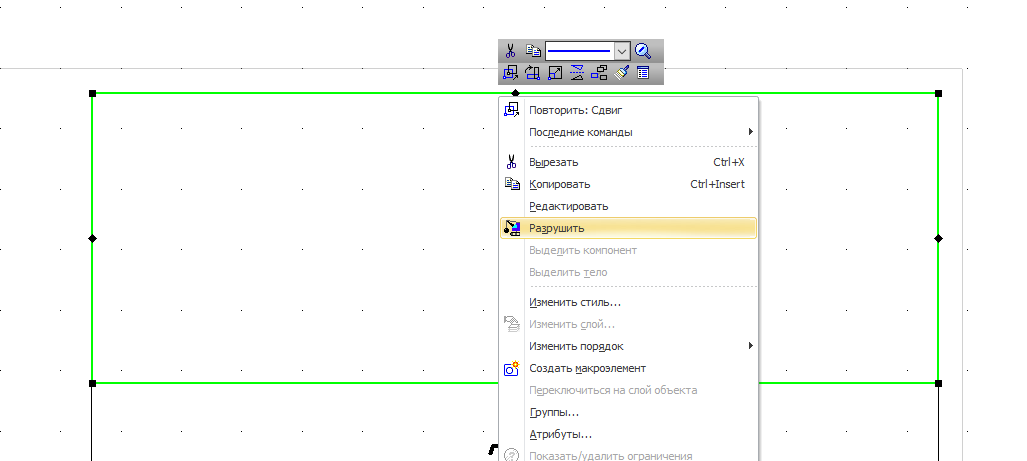
\includegraphics[width=0.9\linewidth]{./images/lab3/step3.png}
    \caption{Застосування інструменту ``Зруйнувати''}
    \label{fig:lab3:dismantle} 
  \end{figure}
\item За допомогою інструменту ``Дуга'', будуємо дугу з вказаним радіусом (\ref{fig:lab3:step3}).
  \begin{figure}[!ht]
    \centering 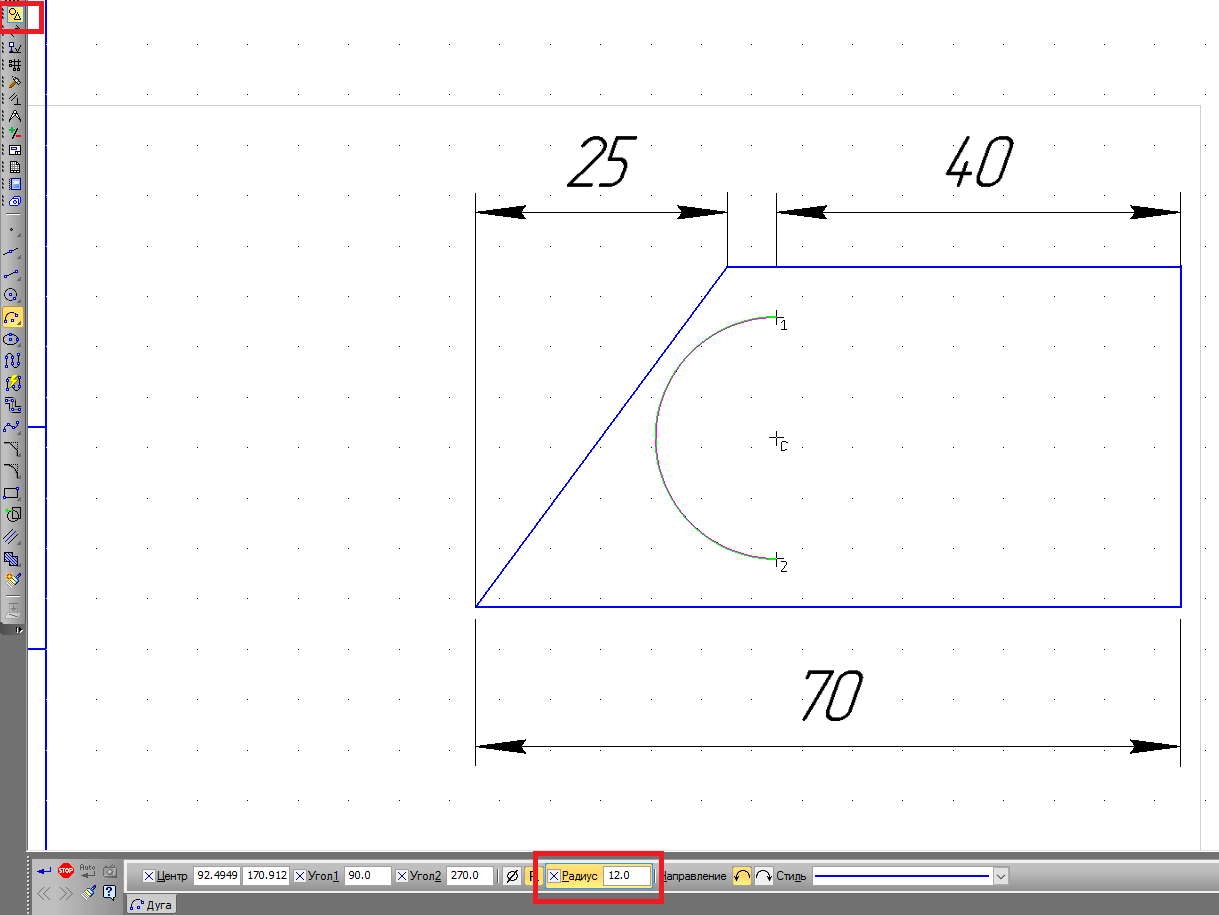
\includegraphics[width=0.9\linewidth]{./images/lab3/step4.png}
    \caption{Застосування інструменту ``Дуга''}
    \label{fig:lab3:step3} 
  \end{figure}

\item Використовуючи інструмент ``Лінія між двома точками'', будуємо осоьову лінію
  (\ref{fig:lab3:central_line}) та допрацьовуємо внутрішній контур клесленика
  (\ref{fig:lab3:step6}).
  \begin{figure}[!ht]
    \centering 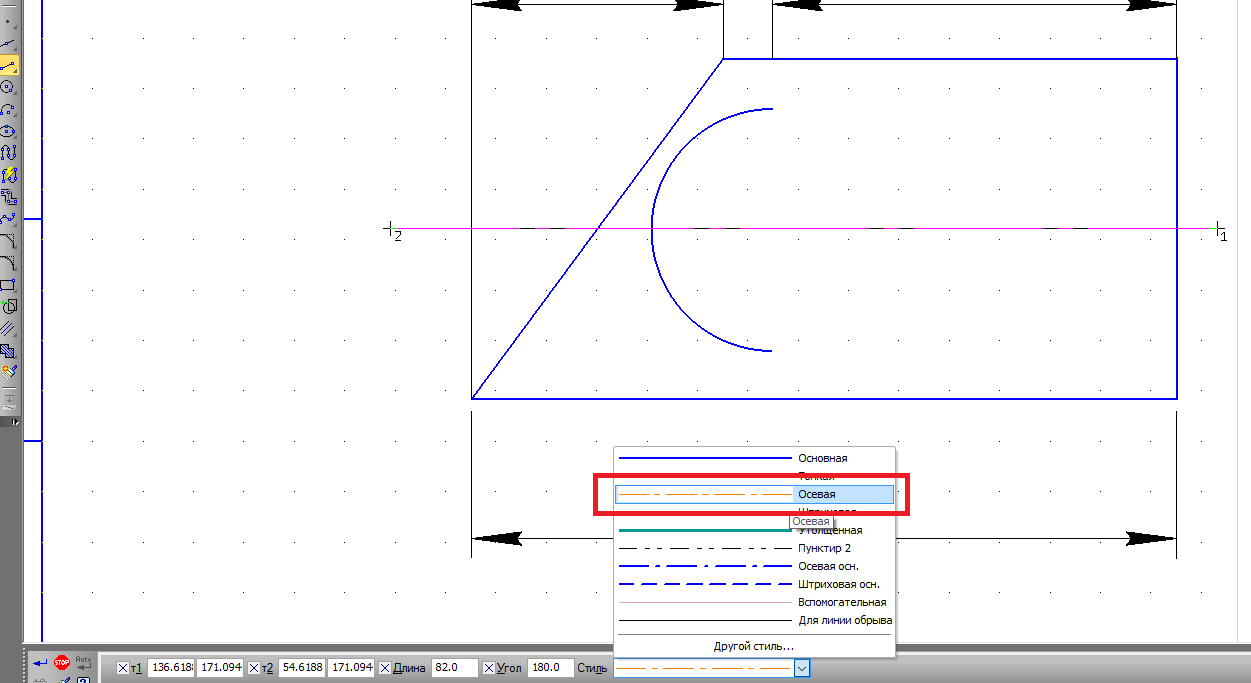
\includegraphics[width=0.9\linewidth]{./images/lab3/step5.png}
    \caption{Застосування інструменту ``Лінія між двома точками''}
    \label{fig:lab3:central_line} 
  \end{figure}
  \begin{figure}[!ht]
    \centering 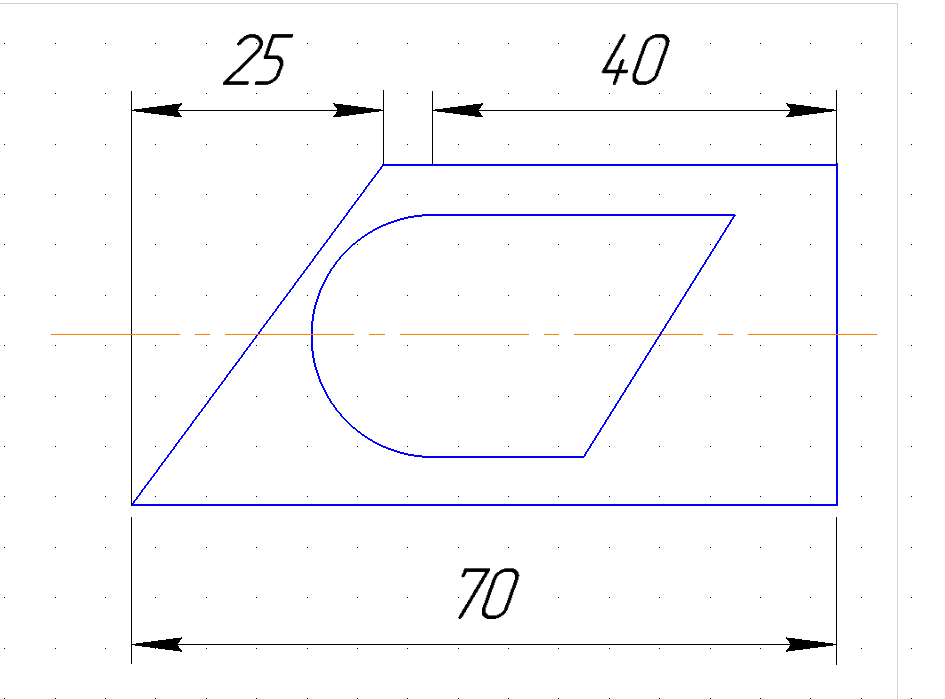
\includegraphics[width=0.9\linewidth]{./images/lab3/step6.png}
    \caption{\label{fig:lab3:step6}}
  \end{figure}

  \newpage
\item Інструментом ``Радіальний розмір'' вказуємо розміри дуги. (\ref{fig:lab3:radial_dimentions}).
  \begin{figure}[!ht]
    \centering 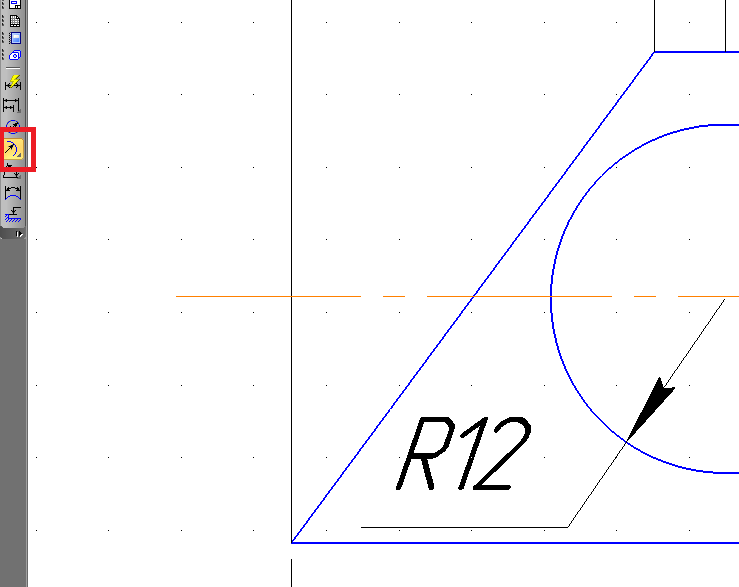
\includegraphics[width=0.9\linewidth]{./images/lab3/step7.png}
    \caption{Застосування інструменту ``Радіальний розмір''}
    \label{fig:lab3:radial_dimentions} 
  \end{figure}

\end{enumerate}

\FloatBarrier Готовий кресленик навадений на сторінці \pageref{lab3:pdf:drawing}.
\newpage
\NoBgThispage
\label{lab3:pdf:drawing}
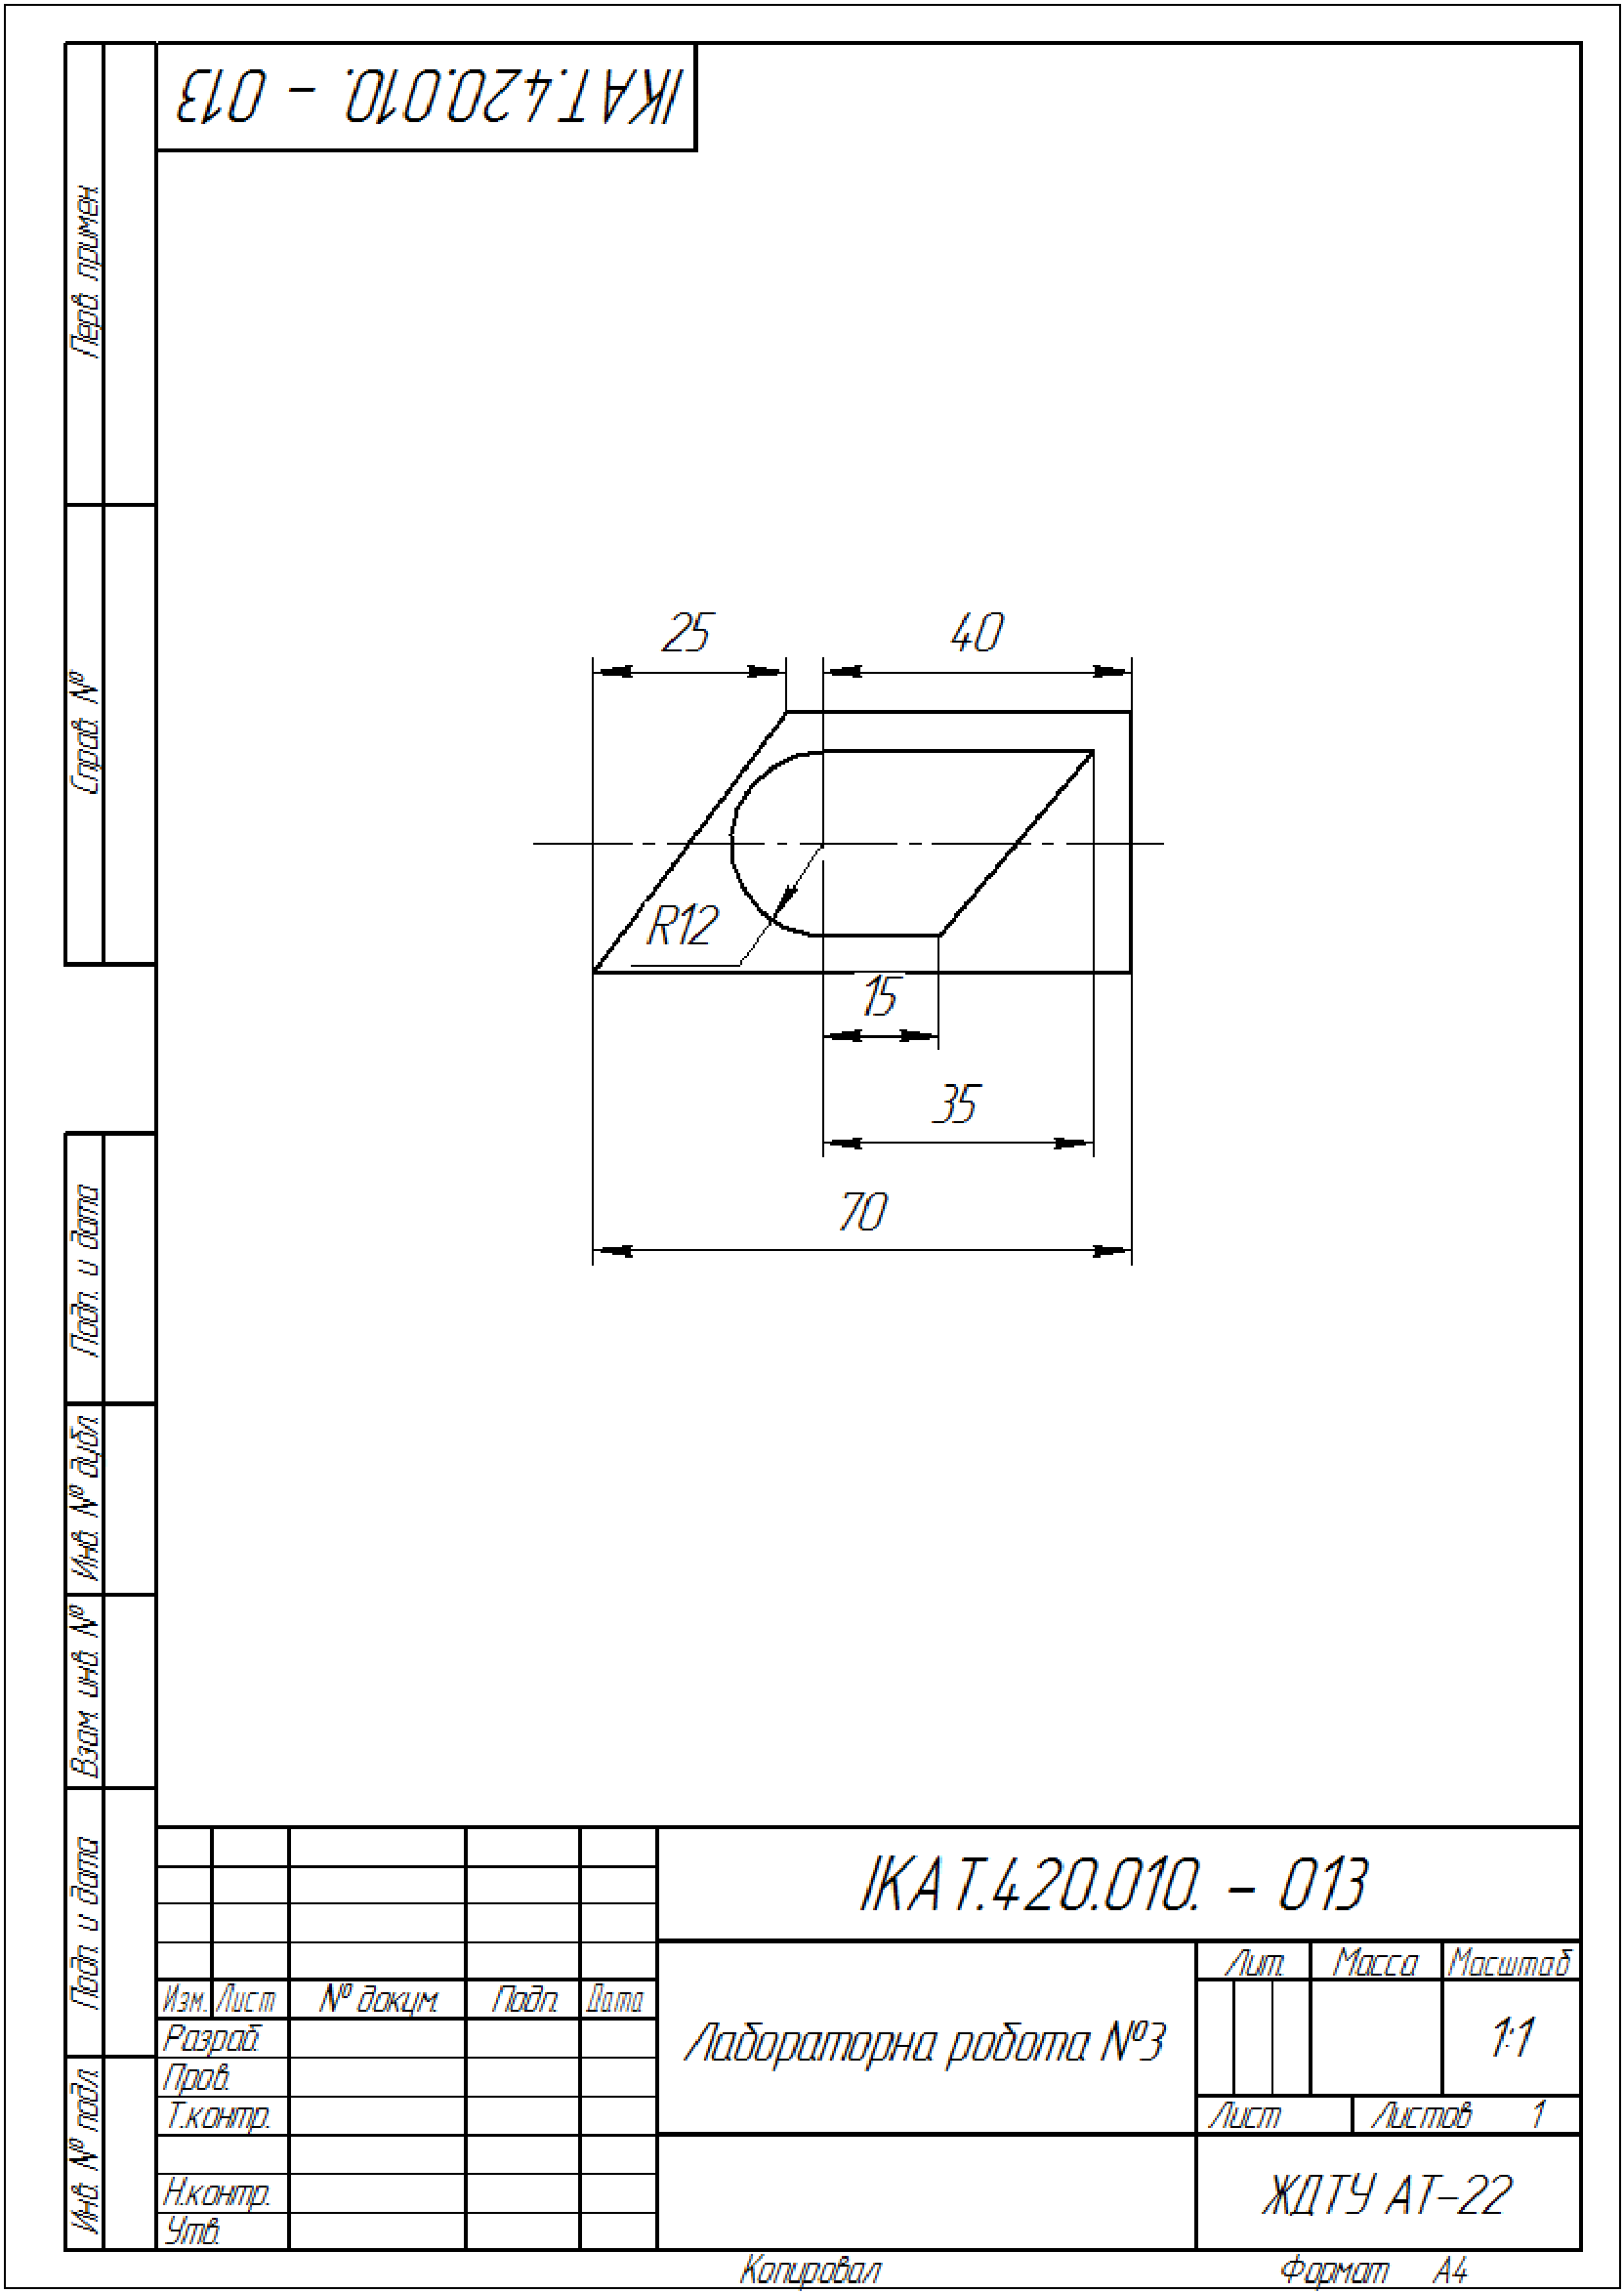
\includepdf{./src/lab3/drawing.pdf} \BorderText

\newpage
\section*{Висновки}

\textbf{КОМПАС 3D} --- потужний програмний пакет, що дозволяє створювати, креслення та інженерну
документацію різної складності.

В ході виконання даної роботи, було проведено ознайомлення з
базовими інструментами програми. З використанням цих інструментів було побудовано задану за
варіантом деталь.
